\section{Implementierung analoger Regler}

\textbf{Voraussetung:} Regler ist ausgelegt (Parameter und Struktur des Reglers bekannt)


\subsection{Struktur allgemeiner Frequenzgang eines Reglers}

Der Frequenzgang des Reglers $G_R(\jimg \omega)$ mit ($m \leq n$) ist beschrieben durch
$$ G_R(\jimg \omega) = \frac{U(\jimg \omega)}{E(\jimg \omega)} 
    = \frac{b_n (\jimg \omega)^n + b_{n-1}(\jimg \omega)^{n-1} + \ldots + b_0}{(\jimg \omega)^n + a_{n-1}(\jimg \omega)^{n-1} + \ldots + a_0} 
    = \frac{b_n + b_{n-1} \frac{1}{\jimg \omega} + \ldots + b_0 \frac{1}{(\jimg \omega)^n}}{1 + a_{n-1} \frac{1}{\jimg \omega} + \ldots + a_0 \frac{1}{(\jimg \omega)^n}} $$

\begin{minipage}[c]{0.55\columnwidth}
    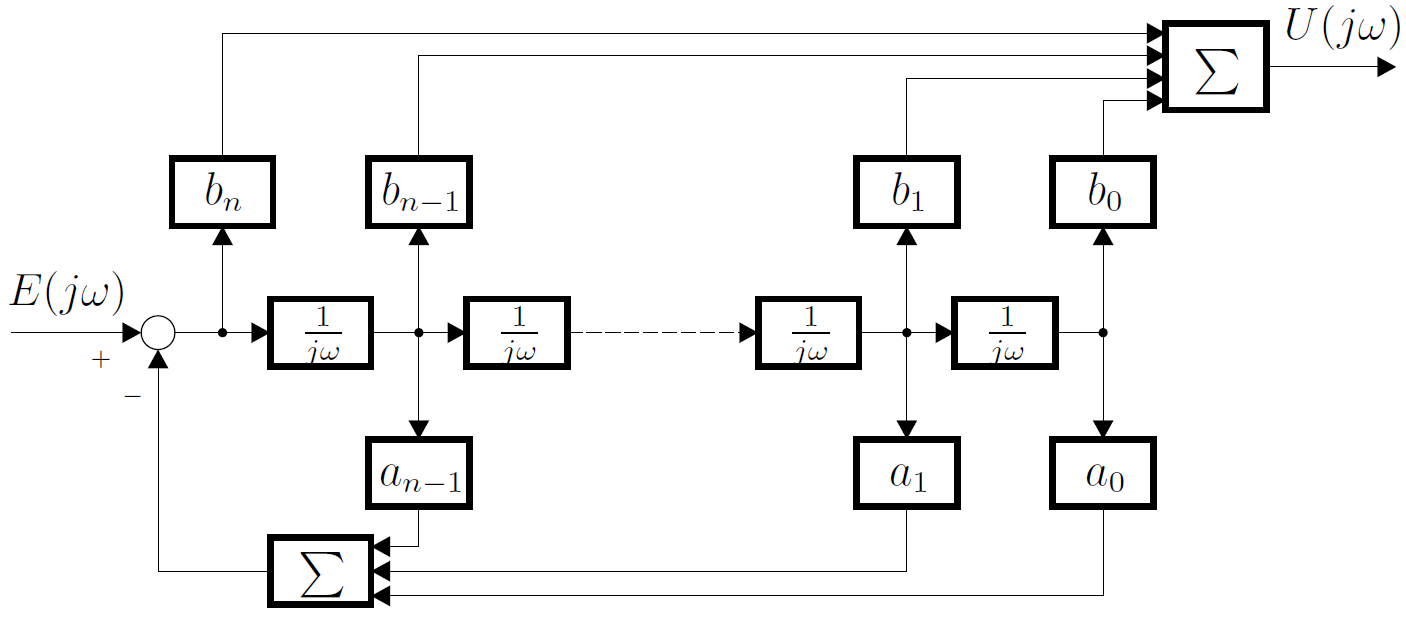
\includegraphics[width=\columnwidth]{images/struktur_allgemeiner_frequenzgang.png}
\end{minipage}
\hfill
\begin{minipage}[c]{0.43\columnwidth}
    Ein jeder solcher Frequenzgang besteht nur aus \textbf{Integratoren, Summatoren und Verstärkungen}. 
    Diese Grundglieder können mit OpAmp-Schaltungen realisiert werden.
\end{minipage}


\subsection{Grundschaltungen mit OpAmps}

\textbf{Hinweis:} Die folgenden Betrachtungen gelten für \textbf{ideale OpAmps}!


\subsubsection{Summator}

\begin{minipage}[c]{0.35\columnwidth}
    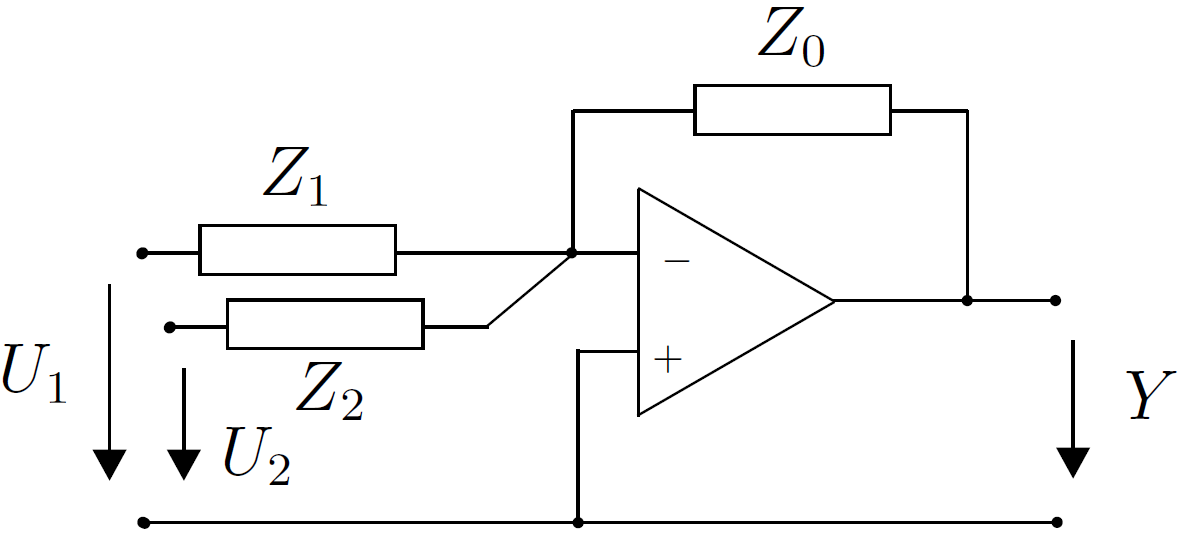
\includegraphics[width=\columnwidth]{images/opamp_grundschaltung_2_eingaenge.png}
\end{minipage}
\hfill
\begin{minipage}[c]{0.62\columnwidth}
    % \raggedright
    $$ Y = - \frac{Z_0}{Z_1} \cdot U_1 - \frac{Z_0}{Z_2} \cdot U_2 $$
    \textrightarrow Auf beliebig viele Eingaänge erweiterbar
\end{minipage}


\subsubsection{Integrierer}

\begin{minipage}[c]{0.35\columnwidth}
    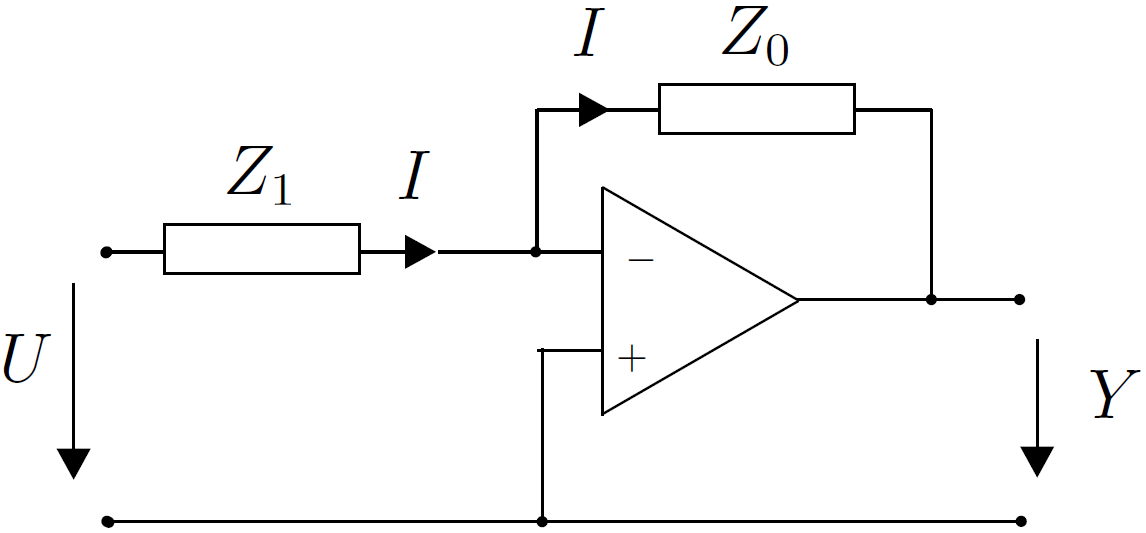
\includegraphics[width=\columnwidth]{images/opamp_grundschaltung_1_eingang.png}
\end{minipage}
\hfill
\begin{minipage}[c]{0.62\columnwidth}
    $$ Z_0 = \frac{1}{\jimg \omega C} \text{ (Kondensator) } \qquad  Z_1 = R $$
    $$ Y = - \frac{1}{\jimg \omega R C} \cdot U \quad \Rightarrow Y =  - \frac{1}{\jimg \omega R_1 C} \cdot U_1 - \frac{1}{\jimg \omega R_2 C} \cdot U_2 $$
\end{minipage}          

\vspace{0.2cm}
\begin{itemize}
        \item Für einen oder mehrere Eingänge geeignet
        \item Braucht 'Reset'-Schaltung, um Kondensator zu entladen
        \item \textbf{Anti-Wind-Up} durch Sättigung der Speisespannung \textbf{gegeben}
\end{itemize}


\subsubsection{P-Glied (passiv)}

\begin{minipage}[c]{0.28\columnwidth}
    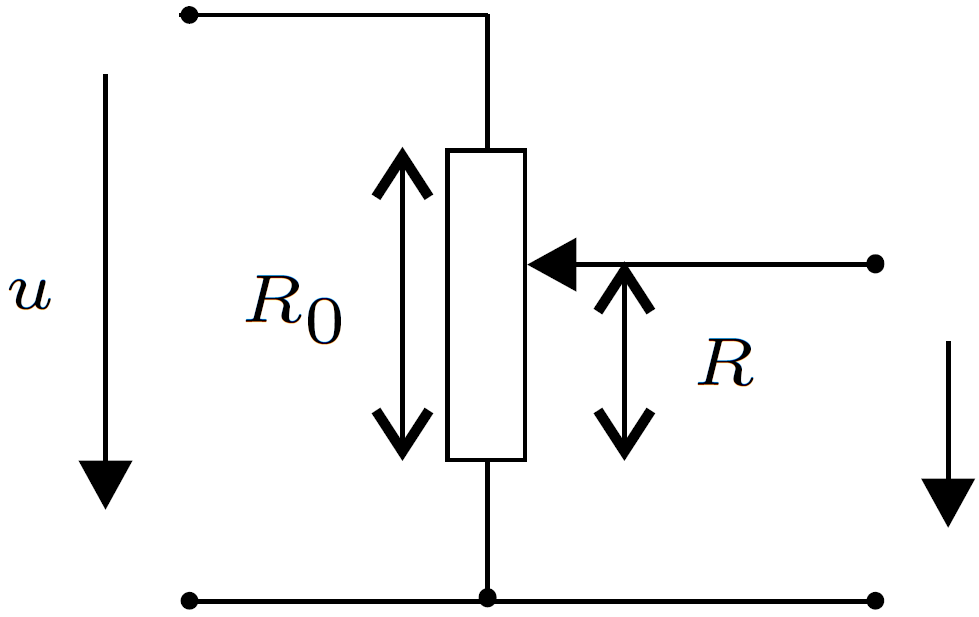
\includegraphics[width=\columnwidth]{images/spannungsteiler.png}
\end{minipage}
\hfill
\begin{minipage}[c]{0.7\columnwidth}
    % $$ y = u \cdot \frac{R}{R_0} $$

    \begin{tabular}{ll}
        Verstärkung $< 1$  & \textrightarrow\ passiver Spannungsteiler \\
        Verstärkung $> 1$  & \textrightarrow\ OpAmp-Schaltung \\
    \end{tabular}

    \vspace{0.2cm}

    \begin{itemize}
        \item OpAmps sollten als Summierer oder Integratoren mit definierter Verstärkung aufgebaut werden
        \item Vor Eingänge des OpAmps passive Spannungsteiler setzen
    \end{itemize}
\end{minipage}


\subsection{Varianten analoger PID-Schaltungen}

\subsubsection{Variante 1 (gemischt)}

\begin{minipage}[c]{0.48\columnwidth}
    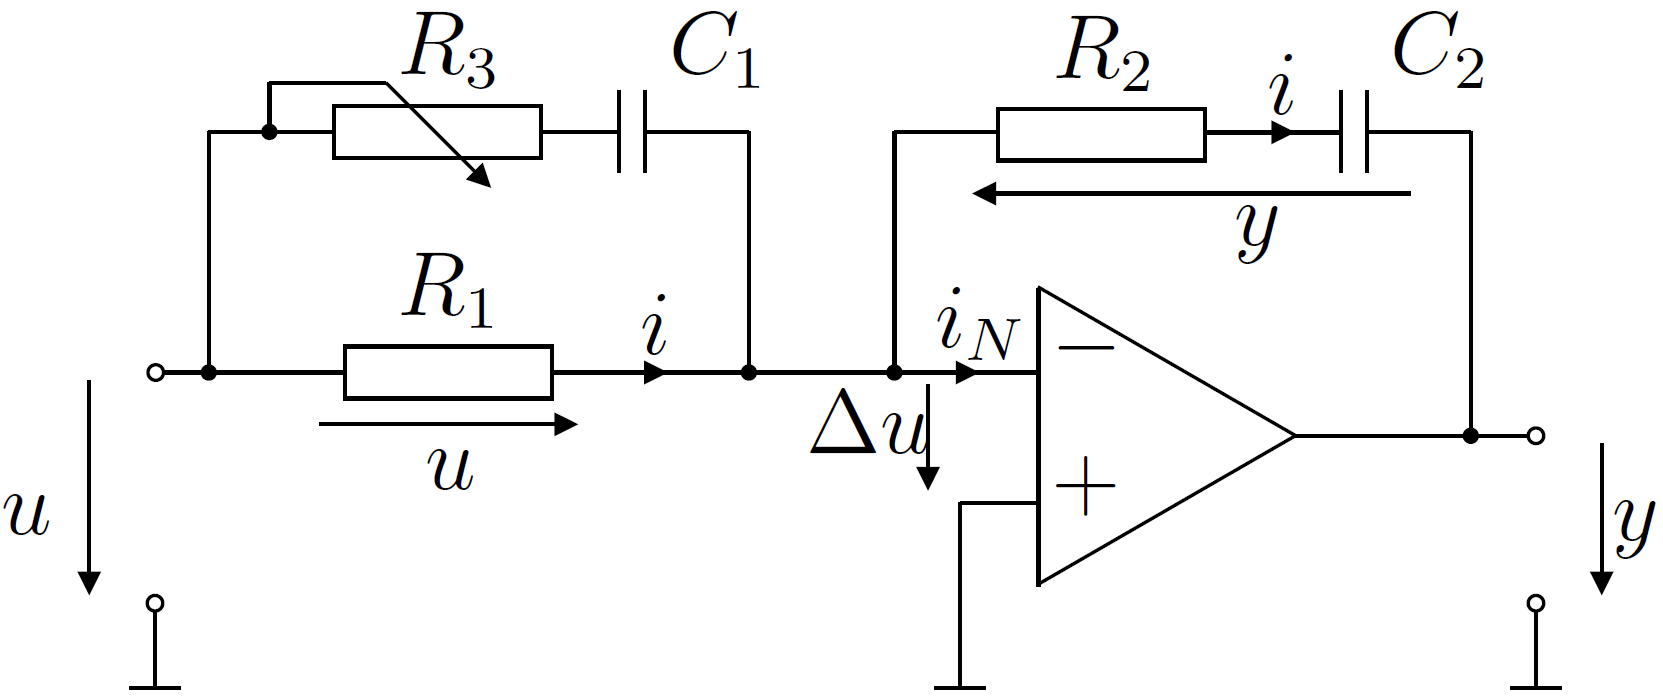
\includegraphics[width=\columnwidth]{images/realisierung_pid-regler_variante_1.png}
\end{minipage}
\hfill
\begin{minipage}[c]{0.48\columnwidth}
    \begin{tabular}{ll}
        $R_1$   & Proportional (P-Anteil) \\
        $C_1$   & Ableitung (D-Anteil) \\
        $R_3$   & Filterkonstante der Ableitung \\
                & \textrightarrow $R_1$ und $C_1$ bilden $\text{DT}_1$-Anteil \\
        $C_2$   & Integral (I-Anteil) \\
    \end{tabular}
    \vspace{0.2cm}

    \textrightarrow Betrachtung als Summator mit $Z_0$ und $Z_1$ möglich
\end{minipage}


\subsubsection{Variante 2 (Parallelform)}

\begin{minipage}[c]{0.45\columnwidth}
    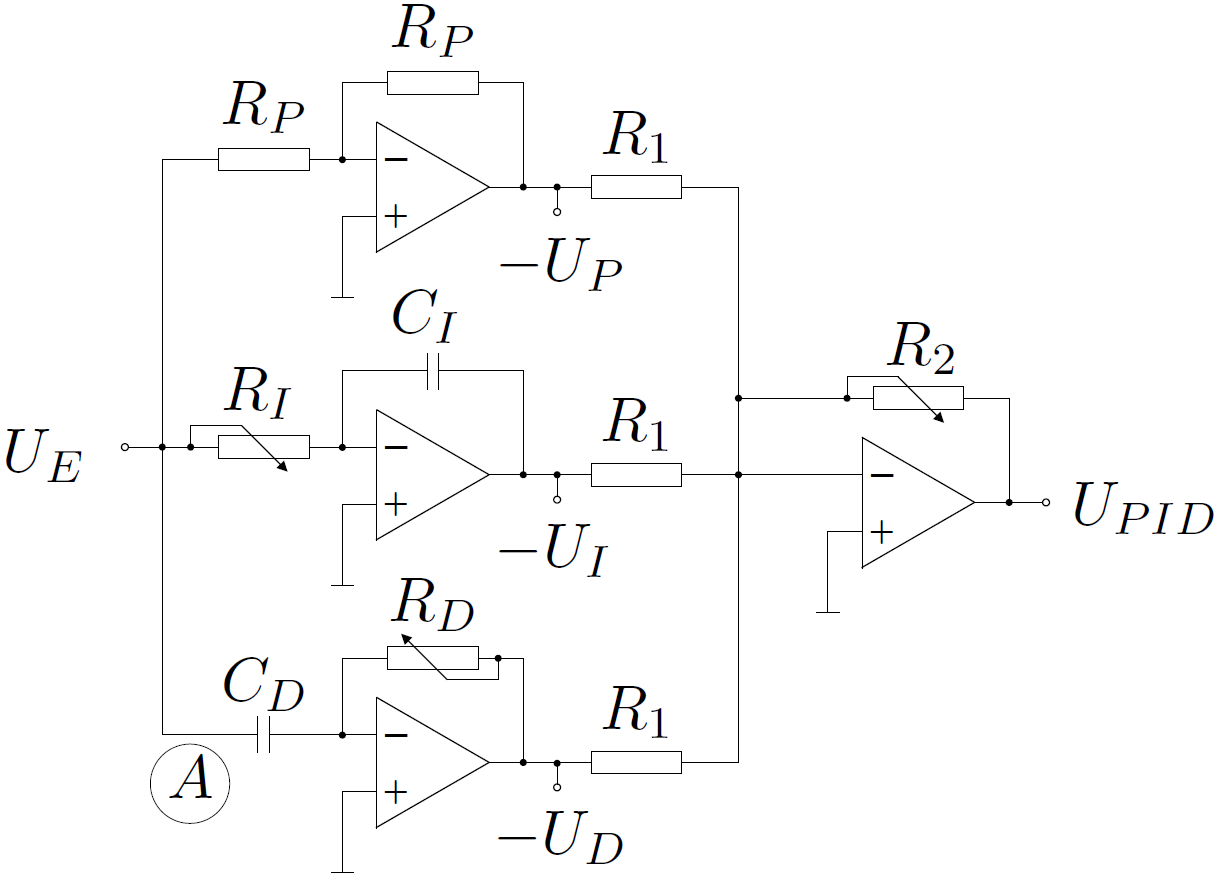
\includegraphics[width=\columnwidth]{images/realisierung_pid-regler_variante_2.png}
\end{minipage}
\hfill
\begin{minipage}[c]{0.52\columnwidth}
    Der Frequenzgang $G(\jimg \omega)$ des Reglers lautet
    $$ \frac{U_{\rm PID}}{U_E} = \underbrace{ \frac{R_2}{R_1} }_{K_R} \cdot \Bigg\lgroup 1 + \frac{1}{\jimg \omega \underbrace{C_I R_I}_{T_N}} 
        + \jimg \omega \underbrace{ C_D R_D }_{T_V} \Bigg\rgroup $$
    Durch Einbau eines Widerstands an der Stelle \textbf{A} wird der der PID-Regler zu einem $\text{PIDT}_1$-Regler.
\end{minipage}

